\documentclass[a4paper,twoside,11pt]{article}
\usepackage{a4wide,graphicx,fancyhdr,amsmath,amssymb, enumerate, caption, subcaption, wrapfig}

%----------------------- Macros and Definitions --------------------------

\setlength\headheight{20pt}
\addtolength\topmargin{-10pt}
\addtolength\footskip{20pt}

\newcommand{\HRule}{\rule{\linewidth}{0.5mm}} % Defines a new command for the horizontal lines,
\newcommand{\N}{\mathbb{N}}
\newcommand{\ch}{\mathcal{CH}}

\fancypagestyle{plain}
\fancyhf{}
\fancyhead[LO,RE]{\sffamily\bfseries\large Technische Universiteit Eindhoven}
\fancyhead[RO,LE]{\sffamily\bfseries\large 2IV35 Visualization}
\fancyfoot[LO,RE]{\sffamily\bfseries\large Department of Mathematics and Computer Science}
\fancyfoot[RO,LE]{\sffamily\bfseries\thepage}
\renewcommand{\headrulewidth}{0pt}
\renewcommand{\footrulewidth}{0pt}


\pagestyle{fancy}
\fancyhf{}
\fancyhead[RO,LE]{\sffamily\bfseries\large Technische Universiteit Eindhoven}
\fancyhead[LO,RE]{\sffamily\bfseries\large 2IV35 Visualization}
\fancyfoot[LO,RE]{\sffamily\bfseries\large Department of Mathematics and Computer Science}
\fancyfoot[RO,LE]{\sffamily\bfseries\thepage}
\renewcommand{\headrulewidth}{1pt}
\renewcommand{\footrulewidth}{0pt}


\begin{document}
\begin{titlepage}

\center % Center everything on the page

\textsc{\Huge \textbf{Technische Universiteit Eindhoven}}\\[1.5cm] % Name of your university/college
\textsc{\LARGE \textbf{Visualization}}\\[0.5cm] % Major heading such as course name
\textsc{\large 2IV35}\\[0.5cm] % Minor heading such as course title

\HRule \\[0.4cm]
{ \huge \bfseries Visualization data of Inflammation}\\[0.4cm] % Title of your document
\HRule \\[1.5cm]

\begin{minipage}{0.4\textwidth}
\begin{flushleft} \large
\emph{\textbf{Author:}}\\
Sander Kools \\
0848523 \\
s.w.a.kools@student.tue.nl % Your name
\end{flushleft}
\end{minipage}
~
\begin{minipage}{0.4\textwidth}
\begin{flushright} \large
\emph{\textbf{Author:}}\\
Luuk Hulten\\
0720248 \\
l.a.j.v.hulten@student.tue.nl
\end{flushright}
\end{minipage}\\[4cm]

{\large \today}\\[3cm] % Date, change the \today to a set date if you want to be precise

\vfill % Fill the rest of the page with whitespace

\end{titlepage}

\section*{Information Visualization}
In this report we will describe how we implemented a web application for visualizing a large data set for the course 2IV35. This data contains information about symptoms of patients and the diagnosed disease. \newline
The data available is the temperature, Occurrence of nausea, Lumbar pain, Urine pushing, Micturition pains, Burning of urethra, itch, swelling of urethra outlet, decision: Inflammation of urinary bladder and decision: Nephritis of renal pelvis origin per patient. \newline
In section 1, we will first give a description of the format of the data set. \newline
In section 2, we will explain our design considerations for the interface. \newline
In section 3, we will present our actual implementation, with screenshots and motivation. \newline
Finally in section 4, we will present the conclusion of the visualization.
\begin{figure}[h]
    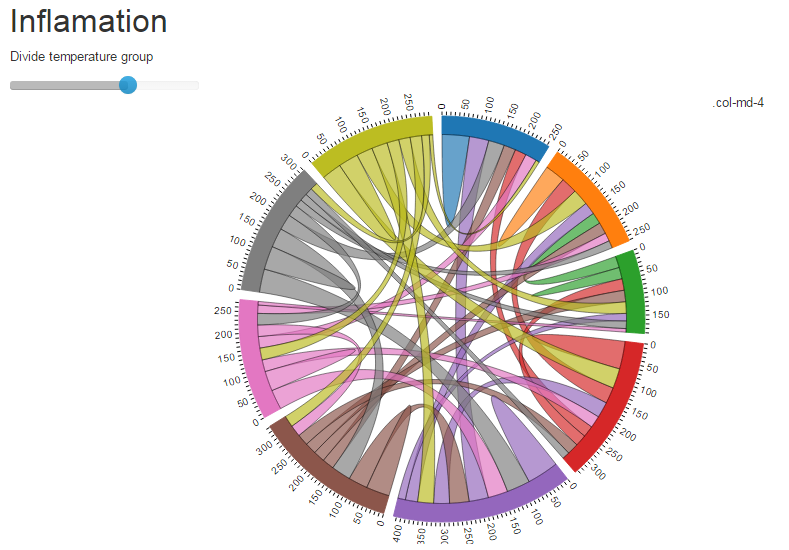
\includegraphics[width=\textwidth]{images/chordDiagram.PNG}
    \caption{the visualization with only the slider ander the chord diagram visible}
    \label{fig:overView}
\end{figure}
\newpage
\section{Description of the Dataset}
We have been given a dataset with information with symptoms and diagnosed deseases. The data is provided in a .csv file with 120 rows and 8 columns every column is separated by a tab. Every row represents a patient. There is also a .txt file with a more detailed explanation on how the data in the .csv can be interpreted.
\subsection{High-level description}
The data set is called "inflammation.csv", the set contains 8 columns that represent the symptoms, and 120 rows of data. The data from the 2nd to the 8th column are "yes" to indicate that he has the disease of that column or "no" to indicate that he doesn't have the disease that the column represents. For example: \newline
\textbf{'35,9 no no yes yes yes yes no'} \newline
Where: \newline
'35,9' Temperature of patient \newline
'no' Occurrence of nausea \newline
'no' Lumbar pain \newline
'yes' Urine pushing (continuous need for urination) \newline
'yes' Micturition pains \newline
'yes' Burning of urethra, itch, swelling of urethra outlet \newline
'yes' decision: Inflammation of urinary bladder \newline
'no' decision: Nephritis of renal pelvis origin  \newline

\subsection{Description of the format}
The data has been gathered from a paper about diagnosis of urinary system diseases \footnote{J.Czerniak, H.Zarzycki, Application of rough sets in the presumptive diagnosis of urinary system diseases, Artifical Inteligence and Security in Computing Systems, ACS'2002 9th International Conference Proceedings, Kluwer Academic Publishers,2003, pp. 41-51} \newline
take from the dataset: \newline
The main idea of this data set is to prepare the algorithm of the expert system, which will perform the presumptive diagnosis of two diseases of urinary system. It will be the example of diagnosing of the acute inflammations of urinary bladder and acute nephritises. For better understanding of the problem let us consider definitions of both diseases given by medics. Acute inflammation of urinary bladder is characterised by sudden occurrence of pains in the abdomen region and the urination in form of constant urine pushing, micturition pains and sometimes lack of urine keeping. Temperature of the body is rising, however most often not above 38C. The excreted urine is turbid and sometimes bloody. At proper treatment, symptoms decay usually within
several days. However, there is inclination to returns. At persons with acute inflammation of urinary bladder, we should expect that the illness will turn into protracted form. \newline
Acute nephritis of renal pelvis origin occurs considerably more often at women than at men. It begins with sudden fever, which reaches, and sometimes exceeds 40C. The fever is accompanied by shivers and one- or both-side lumbar pains, which are sometimes very strong. Symptoms of acute inflammation of urinary bladder appear very often. Quite not infrequently there are nausea and vomiting and spread pains of whole abdomen. \newline
The data was created by a medical expert as a data set to test the expert system, which will perform the presumptive diagnosis of two diseases of urinary system. The basis for rules detection was Rough Sets Theory. Each instance represents an potential patient. \newline
Attribute Information: \newline
a1 Temperature of patient \{ 35C-42C \} \newline
a2 Occurrence of nausea \{ yes, no \} \newline
a3 Lumbar pain \{ yes, no \} \newline
a4 Urine pushing (continuous need for urination) \{ yes, no \} \newline
a5 Micturition pains \{ yes, no \} \newline
a6 Burning of urethra, itch, swelling of urethra outlet \{ yes, no \} \newline
d1 decision: Inflammation of urinary bladder \{ yes, no \} \newline
d2 decision: Nephritis of renal pelvis origin \{ yes, no \} \newline
\newpage
\section{Design}
In this section we explain the general design of the visualization. The goal of the visualization is to find a correlation between symptoms and diagnose. For this multiple visualization , aggregation and filtering techniques can be applied.

\subsection{Visualization techniques}
The data at hand is except of the temperature binary data. In this binary data we have to find patterns or paths to lead to a certain diagnose.
The following visualization techniques where considered:

\subsubsection{Table}
In the table visualization the data is shown in a table. This table can than be filtered and ordered to find patterns in the data.

\begin{itemize}
  \item Pros\\
    Advantages of this technique is that the data is 'pure' the data doesn't need any preprocessing to be visualized.
  \item Cons \\
    A lot of filtering and ordering needs to be applied to find patterns. Also since the quantity of data is quite large it's hard for a person to get a good impression of the data.
\end{itemize}

\subsubsection{Scatter plot}
The scatter plot is a good visualization technique for visualizing lots of data. In this case it would be possible to create a scatter plot with symptoms on the x-axis and patient rows or diagnoses on the y-axis. In a scatter plot clustering and patterns are easily discovered.
\begin{itemize}
  \item Pros\\
    Easy to find patterns \\
    Can display lots of data \\
  \item Cons \\
    Preprocessing of the data is needed in this case \\
    With binary data you get a table like impression of the data \\
\end{itemize}

\newpage

\subsubsection{Box plot}
We can create a statistical interpretation of the data by calculating box plots. For example a good impression of a patient temperature for each diagnose can be given by a box plot.

\begin{itemize}
  \item Pros\\
    Box plots are good in giving statistical data like mean and variance. \\
  \item Cons \\
   Lots of the data is lost in this representation. \\
\end{itemize}

\subsubsection{Chord diagram}
A chord diagram is a visualization method used for displaying relations between data.

\begin{itemize}
  \item Pros\\
    Gives relations between symptoms. \\
    Can display the strength of a relation by the chord sizes.
  \item Cons \\
   Like the scatter plot the data needs pre processing. \\
\end{itemize}

\subsubsection{Parallel Coordinates}
Also the parallel coordinates diagram is particular good in displaying relational data. An advantage of the parallel coordinates visualization technique over the chord diagram is that the data doesn't need preprocessing and also every element in the data could be visualized.

\begin{itemize}
  \item Pros\\
    Can easily show paths in the data. \\
    Most often the data does not need pre-processing. \\
  \item Cons \\
   Is not capable of displaying lots of data. \\
\end{itemize}

\newpage

\subsection{User Interface}
Since the available experience in D3 the choice for a web based D3 approach was easily made. However since the arrival of smart devices people moreover visit web sites with tablets and phones. Thats why the decision for using a responsive design was chosen. Creating a responsive design is very time consuming that so we used bootstrap as a responsive framework. However scaling graphs isn't as easy as we originally thought. Many problems come at hand:
\begin{itemize}
  \item labels aren't readable \\
  \item width height ratio is lost \\
  \item graphs don't wrap nicely beneath each other \\
\end{itemize}
Since there were to many problems and to little time to solve them we dropped the responsive design requirement after applying it on the parallel coordinates graph. \\

Also a slider is created to categorize the temperature in a low and high temperature class. Using this slider the user can shift the temperature in a certain class and search for a point where there is an obvious relation between temperature and diagnose. \\

For the parallel coordinates the category lines are movable. Rearranging these categories can be used to find paths in the data that lead to a diagnose or even to find symptoms that don't have any influence at all on the diagnose. \\

The groups of the Chord diagram are selectable. Selecting a group lets the bar chart displaying the relational data of the selected group. \\
\newpage

\section{Implementation}
For the visualization of data, we used the d3.js library. This library allows developers to visualize data using Javascript easily. Also external library like dimple.js (extention of D3) and bootstrap for responsive design was used.

\subsection{Technical Notes}
We have tested the application in Firefox and Chrome. Other modern browsers like Safari, Opera and Internet Explorer should also support our application.
\subsection{Main Interface}
The main view will be all visualizations below each other with the chord diagram on top, below the parallel coordinates and under that the bar chart, there will be a slider visible on the top of the page on which you can select a temperature range that will filter the data used in the visualizations. These will than update with the filtered data.
\newpage
\subsection{Parallel Coordinates}
We used the dataset that was provided to visualize it in a parallel coordinates visualization. Parallel coordinates are one of the most famous visualization techniques, and among the most common subjects of academic papers in visualization. While initially confusing, they are a very powerful tool for understanding multi-dimensional numerical datasets. \newline
For instance now can be seen that a high temperature and nausea have a direct connection. The full result of this can be seen in figure. \ref{fig:Parallel}.
\begin{figure}[h]
\begin{center}
    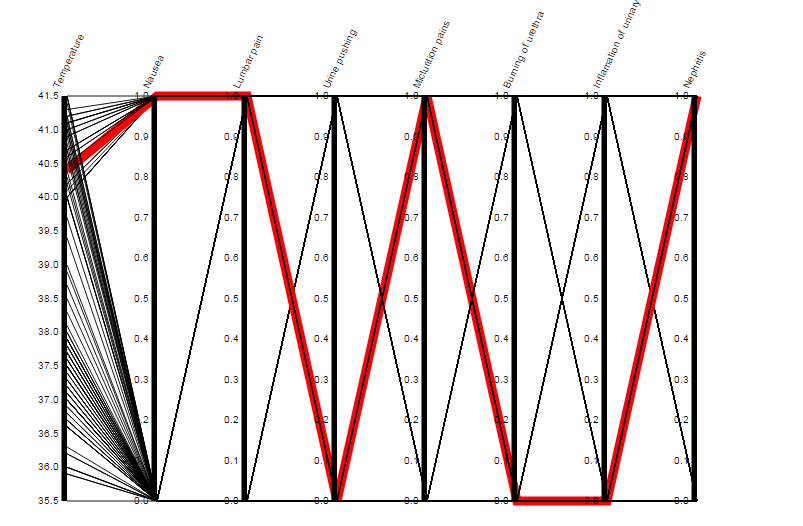
\includegraphics[width=0.8\textwidth]{images/ParallelCoordinates.PNG}
    \caption{the parallel Coordinates visualization}
    \label{fig:Parallel}
\end{center}
\end{figure}
\newpage
\subsection{Bar Chart}
The Bar Chart uses vertical bars to show comparisons among the disease categories. on the x axis the different diseases from the dataset are represented and on the y axis the percentage of people that have it is displayed. The percentage is based on the amount of people that are in the dataset and on which percentage has the disease, for each disease there is a bar. This is a basic technique, but it is very useful to see which diseases are more prevalent among the people. The full result of this can be seen in figure \ref{fig:Bar}.
\begin{figure}[h]
\begin{center}
    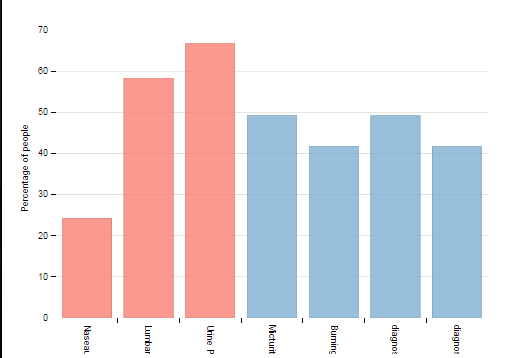
\includegraphics[width=0.8\textwidth]{images/barChart.PNG}
    \caption{the Bar Chart visualization}
    \label{fig:Bar}
\end{center}
\end{figure}
\newpage
\subsection{Chord Diagram}
A chord diagram is a graphical method of displaying the inter-relationships between data in a matrix. The data is arranged radially around a circle with the relationships between the points drawn as arcs connecting the data together. The full result of this visualization can be seen in figure \ref{fig:Chord}\newline. For using the data had to be pre processed to a adjacency matrix. This matrix contains the count that a symptom occurs related to another symptom.
\begin{figure}[h]
\begin{center}
    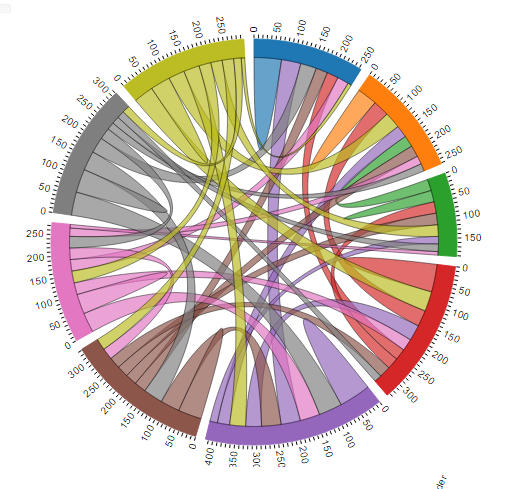
\includegraphics[width=0.8\textwidth]{images/chordDiagramSolo.PNG}
    \caption{the Chord Diagram visualization}
    \label{fig:Chord}
\end{center}
\end{figure}
\newpage
\subsection{Hovering and Selecting}
To get more detail from a particular visualization, the user can hover over it with the mouse, this has an effect on every visualization. \newline
With the chord diagram, just that part of the circle and the relations are highlighted so you can more easily see the relations. \newline
With the parallel coordinates when you hover over a line, it will be highlighted red all along the graph, so you can see how it traverses the graph. \newline
With the bar chart more information of the bar is given if it is hovered over, it will display the full name on the x axis of the disease and also the percentage in a label located at the mouse.

\section{Conclusion}

\subsection{Observation}
With the visualization the influence of symptoms to the resulting treatment can easily be found. Selecting the diagnose in the chord diagram directly shows the dependency on the different symptoms. With the bar chart at the side the influence of each symptom is even better visible.
We can easily observe that patients of Nephritis have a higher temperature accommodated with lumbar pain and nausea.

\begin{figure}[h!]
\begin{center}
    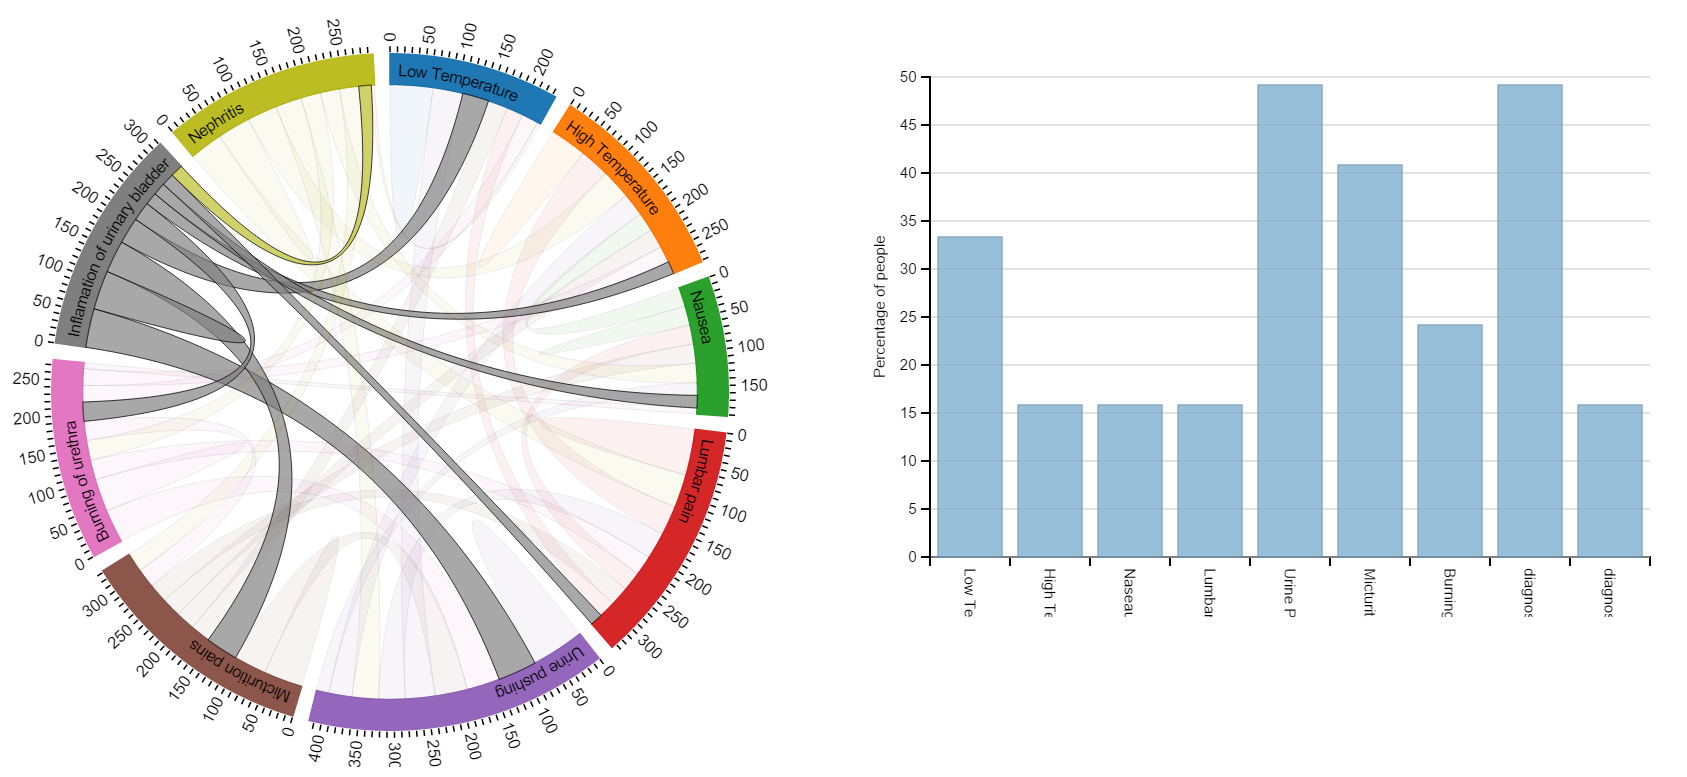
\includegraphics[width=0.8\textwidth]{images/ObservationIoUB.PNG}
    \caption{Observation of diagnose Inflamation of urinary bladder}
    \label{fig:Chord}
\end{center}
\end{figure}

\begin{figure}[h!]
\begin{center}
    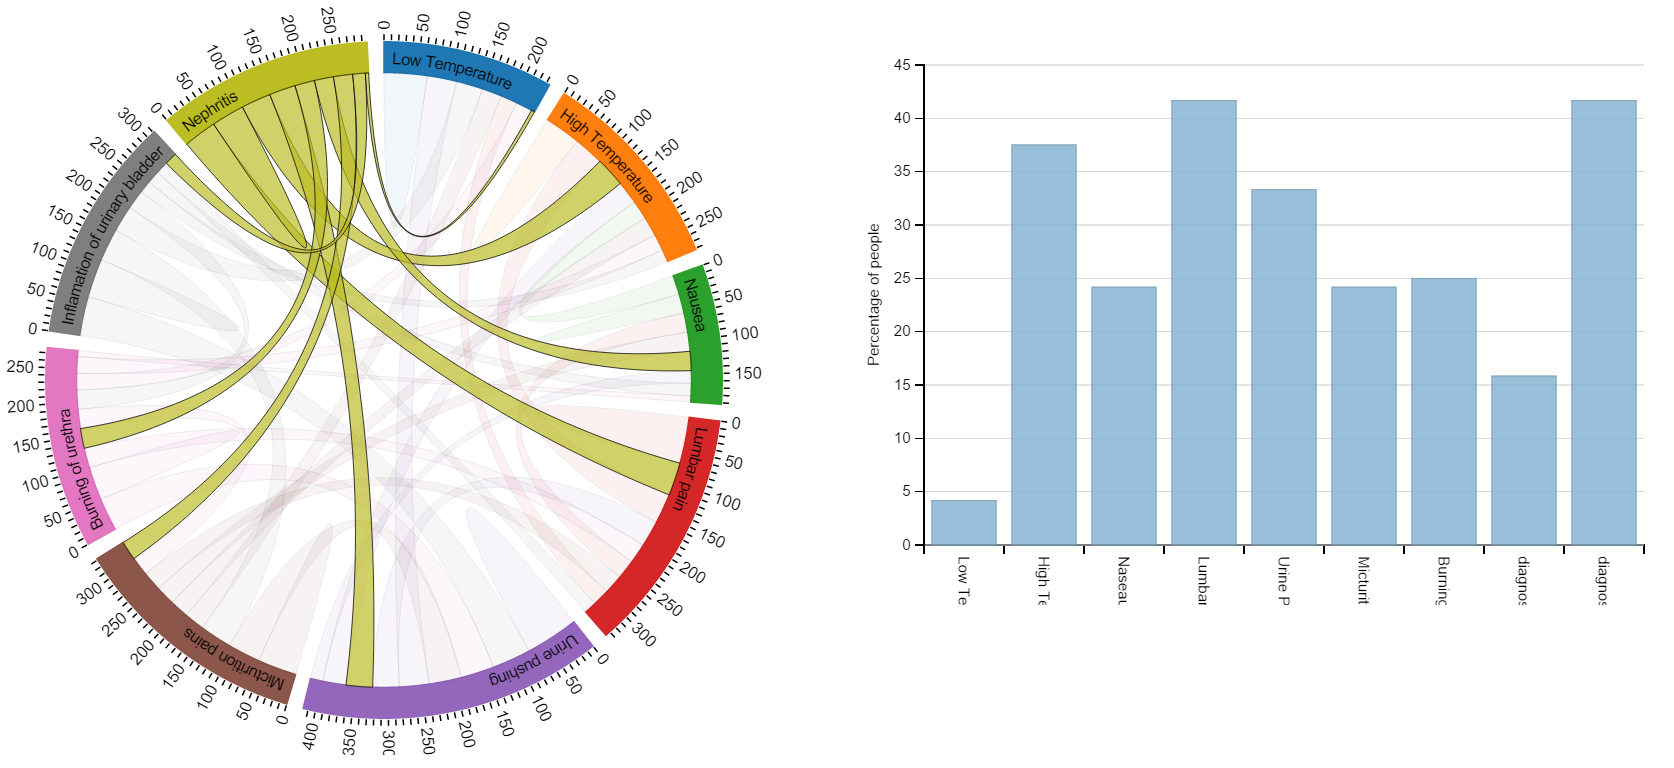
\includegraphics[width=0.8\textwidth]{images/ObservationNephritis.PNG}
    \caption{Observation diagnose Nephritis}
    \label{fig:Chord}
\end{center}
\end{figure}

\subsection{Feedback}
The bar chart and chord chart are very powerfull visualizations for this data. The parallel line graph was not a good choice for visualizing this data. We thought we could easily find paths, leading to a certain diagnose. However, since the data consist mostly out of binary data all lines are drawn on top of each other. This prevents the user to distinct different lines in the view. 

We have a slider for changing the temperature group data. The user has to set this intuitively. A good idea would be to implement a box plot graph. This graph should contain a plot for each symptom per diagnose. From this the user could directly find good setting values and iterate from that.

Another thing for improvement is removing the scale change when selecting an other group data from the chord. By rescaling the y-axis the user loses his view on the new values compared to the previous ones.

Work breakdown:
Responsiveness: Sander, Luuk
Bar chart: Sander
Chord chart: Luuk
Parallel line: Luuk
Animations: Sander

\end{document} 